\chapter{Qweak Simulation General Structure and Compile Information}\label{CHP_I}

\section{Class Structure} \label{CHP_I-SCN_I}

Tables~\ref{tbl:classlist1} through \ref{tbl:classlist3} show the list of
C++ source and header files currently included in the simulation.
Every class or object in the program {\bf always} has a header and
source file in which the class declaration and implementation are
separated from each other. This enhances readability and organization.

Not all of theses classes are currently used in the \textit{QweakSimG4}
program. The dictionary files (xxxDict.h or xxxDict.cc) are
automatically generated by ROOT (see ~\cite{tn:ROOT}) and should not
be edited. The classes {\em QweakSimMagnetFieldMapMessenger}, {\em
QweakSimMiniMagnetMessenger}, {\em QweakSimSteppingVerbose}, and {\em
QweakSimTrajectory} are available but currently not used.  Most of the
{\em QweakSimG4} classes are derived, i.e. inherit some of their
properties, from a small number of GEANT4 classes and some of the base
classes are ROOT extensions.

\begin{landscape}
\begin{table}
\begin{center}
\begin{tabular}{ll}
\hline 
{\bf Header}                  &  {\bf Source}               \\
\hline 
 QweakSimAnalysis.hh                                & QweakSimAnalysis.cc                                          \\
 QweakSimCerenkovDetector.hh                        & QweakSimCerenkovDetector.cc                                  \\
 QweakSimCerenkov\_DetectorHit.hh                   & QweakSimCerenkov\_DetectorHit.cc                              \\
 QweakSimCerenkovDetectorMessenger.hh               & QweakSimCerenkovDetectorMessenger.cc                         \\
 QweakSimCerenkovDetector\_PMTHit.hh                & QweakSimCerenkovDetector\_PMTHit.cc                           \\
 QweakSimCerenkovDetector\_PMTSD.hh                 & QweakSimCerenkovDetector\_PMTSD.cc                            \\
 QweakSimCerenkov\_DetectorSD.hh                    & QweakSimCerenkov\_DetectorSD.cc                               \\
 QweakSimCollimator.hh                              & QweakSimCollimator.cc                                        \\
 QweakSimCollimatorSupport.hh                       & QweakSimCollimatorSupport.cc                                 \\
 QweakSimDetectorConstruction.hh                    & QweakSimDetectorConstruction.cc                              \\
 QweakSimDetectorMessenger.hh                       & QweakSimDetectorMessenger.cc                                 \\
 QweakSimEventAction.hh                             & QweakSimEventAction.cc                                       \\
 QweakSimG3Ntuple.hh                                & QweakSimG3Ntuple.cc                                          \\
 QweakSimG3NtupleReader.hh                          & QweakSimG3NtupleReader.cc                                    \\
 QweakSimGEM.hh 				    & QweakSimGEM.cc                 	                           \\
 QweakSimGEMMessenger.hh 			    & QweakSimGEMMessenger.cc        	                           \\
 QweakSimGEM\_WirePlaneHit.hh			    & QweakSimGEM\_WirePlaneHit.cc                                  \\
 QweakSimGEM\_WirePlaneSD.hh			    & QweakSimGEM\_WirePlaneSD.cc                                   \\
 QweakSimGlobalMagnetField.hh                       & QweakSimGlobalMagnetField.cc                                 \\
 QweakSimHDC.hh                                     & QweakSimHDC.cc                                               \\        
 QweakSimHDCMessenger.hh             		    & QweakSimHDCMessenger.cc                                      \\
 QweakSimHDC\_WirePlaneHit.hh         		    & QweakSimHDC\_WirePlaneHit.cc                                   \\
 QweakSimHDC\_WirePlaneSD.hh          		    & QweakSimHDC\_WirePlaneSD.cc                                    \\
 QweakSimInputRootFile\_EventReader.hh		    & QweakSimInputRootFile\_EventReader.cc                         \\
 QweakSimMagnet\_CoilParameterisation.hh            & QweakSimMagnet\_CoilParameterisation.cc                       \\
 QweakSimMagnetFieldMap.hh                          & QweakSimMagnetFieldMap.cc                                    \\
 QweakSimMagnetFieldMapMessenger.hh                 & QweakSimMagnetFieldMapMessenger.cc                           \\
\hline
\end{tabular}
\end{center}
\caption{List of classes}
\label{tbl:classlist1}
\end{table}

\clearpage

\begin{table}
\begin{center}
\begin{tabular}{ll}
\hline 
 {\bf Header}                  &  {\bf Source}               \\
\hline 
 QweakSimMagnet\_MiniTorusCoilParameterisation.hh   & QweakSimMagnet\_MiniTorusCoilParameterisation.cc              \\
 QweakSimMainMagnet.hh                              & QweakSimMainMagnet.cc                                        \\
 QweakSimMaterial.hh                                & QweakSimMaterial.cc                                          \\
 QweakSimMiniMagnet.hh                              & QweakSimMiniMagnet.cc                                        \\
 QweakSimMiniMagnetMessenger.hh                     & QweakSimMiniMagnetMessenger.cc                               \\
 QweakSimPhysicsList.hh                             & QweakSimPhysicsList.cc                                       \\
 QweakSimPhysicsListMessenger.hh                    & QweakSimPhysicsListMessenger.cc                              \\
 QweakSimPrimaryGeneratorAction.hh                  & QweakSimPrimaryGeneratorAction.cc                            \\
 QweakSimPrimaryGeneratorActionMessenger.hh         & QweakSimPrimaryGeneratorActionMessenger.cc                   \\
 QweakSimRunAction.hh                               & QweakSimRunAction.cc                                         \\
 QweakSimShieldingWall.hh                           & QweakSimShieldingWall.cc                                     \\
 QweakSimShieldingWallMessenger.hh                  & QweakSimShieldingWallMessenger.cc                            \\
 QweakSimStackingAction.hh                          & QweakSimStackingAction.cc                                    \\
 QweakSimSteppingAction.hh                          & QweakSimSteppingAction.cc                                    \\
 QweakSimSteppingVerbose.hh                         & QweakSimSteppingVerbose.cc                                   \\
 QweakSimTarget.hh                                  & QweakSimTarget.cc                                            \\
 QweakSimTargetMessenger.hh                         & QweakSimTargetMessenger.cc                                   \\
 QweakSimTrackHistory.hh                            & QweakSimTrackHistory.cc                                      \\     
 QweakSimTrackInformation.hh                        & QweakSimTrackInformation.cc                                  \\
 QweakSimTrackingAction.hh                          & QweakSimTrackingAction.cc                                    \\
 QweakSimTrackingActionMessenger.hh                 & QweakSimTrackingActionMessenger.cc                           \\
 QweakSimTrajectory.hh                              & QweakSimTrajectory.cc                                        \\
 QweakSimTriggerScintillator.hh                     & QweakSimTriggerScintillator.cc                               \\     
 QweakSimTriggerScintillator\_DetectorHit.hh        & QweakSimTriggerScintillator\_DetectorHit.cc                   \\
 QweakSimTriggerScintillator\_DetectorSD.hh         & QweakSimTriggerScintillator\_DetectorSD.cc                    \\
 QweakSimTriggerScintillatorMessenger.hh            & QweakSimTriggerScintillatorMessenger.cc                       \\
 QweakSimUserCerenkov\_DetectorEvent.hh             & QweakSimUserCerenkov\_DetectorEvent.cc                        \\
\hline
\end{tabular}
\end{center}
\caption{List of classes}
\label{tbl:classlist2}
\end{table}
\end{landscape}
\clearpage


\begin{landscape}
\begin{table}
\begin{center}
\begin{tabular}{ll}
\hline 
 {\bf Header}                  &  {\bf Source}               \\
\hline 
 QweakSimUserCerenkov\_MainEvent.hh                 & QweakSimUserCerenkov\_MainEvent.cc                            \\
 QweakSimUserCerenkov\_OctantEvent.hh               & QweakSimUserCerenkov\_OctantEvent.cc                         \\
 QweakSimUserCerenkov\_PMTEvent.hh                  & QweakSimUserCerenkov\_PMTEvent.cc                             \\
 QweakSimUserGEM\_MainEvent.hh                      & QweakSimUserGEM\_MainEvent.cc          \\   
 QweakSimUserGEM\_SingleGEMEvent.hh                 & QweakSimUserGEM\_SingleGEMEvent.cc     \\
 QweakSimUserGEM\_WirePlaneEvent.hh                 & QweakSimUserGEM\_WirePlaneEvent.cc     \\
 QweakSimUserHDC\_MainEvent.hh                      & QweakSimUserHDC\_MainEvent.cc          \\        
 QweakSimUserHDC\_SingleHDCEvent.hh                 & QweakSimUserHDC\_SingleHDCEvent.cc     \\
 QweakSimUserHDC\_WirePlaneEvent.hh                 & QweakSimUserHDC\_WirePlaneEvent.cc     \\
 QweakSimUserInformation.hh                         & QweakSimUserInformation.cc                                   \\
 QweakSimUserMainEvent.hh                           & QweakSimUserMainEvent.cc                                     \\
 QweakSimUserPrimaryEvent.hh                        & QweakSimUserPrimaryEvent.cc \\                              
 QweakSimUserTriggerScintillator\_DetectorEvent.hh  & QweakSimUserTriggerScintillator\_DetectorEvent.cc \\
 QweakSimUserTriggerScintillator\_MainEvent.hh      & QweakSimUserTriggerScintillator\_MainEvent.cc    \\
 QweakSimUserVDC\_Config.hh                         & QweakSimUserVDC\_Config.cc                                    \\
 QweakSimUserVDC\_DriftCellEvent.hh                 & QweakSimUserVDC\_DriftCellEvent.cc                            \\
 QweakSimUserVDC\_MainEvent.hh                      & QweakSimUserVDC\_MainEvent.cc                                 \\
 QweakSimUserVDC\_SingleVDCEvent.hh                 & QweakSimUserVDC\_SingleVDCEvent.cc                            \\
 QweakSimUserVDC\_WirePlaneEvent.hh                 & QweakSimUserVDC\_WirePlaneEvent.cc                            \\
 QweakSimVDC.hh                                     & QweakSimVDC.cc                                               \\
 QweakSimVDC\_DriftCellBackSD.hh                    & QweakSimVDC\_DriftCellBackSD.cc  \\
 QweakSimVDC\_DriftCellFrontSD.hh                   & QweakSimVDC\_DriftCellFrontSD.cc \\
 QweakSimVDC\_DriftCellHit.hh                       & QweakSimVDC\_DriftCellHit.cc                                  \\
 QweakSimVDC\_DriftCellParameterisation.hh          & QweakSimVDC\_DriftCellParameterisation.cc                     \\
 QweakSimVDCMessenger.hh                            & QweakSimVDCMessenger.cc                                      \\
 QweakSimVDCRotator.hh                              & QweakSimVDCRotator.cc \\ 
 QweakSimVDC\_WirePlaneHit.hh                       & QweakSimVDC\_WirePlaneHit.cc                                  \\
 QweakSimVDC\_WirePlaneSD.hh                        & QweakSimVDC\_WirePlaneSD.cc                                   \\
\hline
\end{tabular}
\end{center}
\caption{List of classes}
\label{tbl:classlist3}
\end{table}
\end{landscape}
\clearpage


Figure~\ref{fig:CLTR1} and~\ref{fig:CLTR2} show the inheritance
structure for the simulation classes. Please refer to the GEANT4
manual on the properties of the base classes. Figure~\ref{fig:CLTR1}
only shows the base classes, some of which are turned into ROOT
objects. All of the ROOT-object {\em QweakSimG4} base classes (shown
in yellow) are event counters which are stored in a ROOT {\em tree}
object after the simulation has completed and must therfore be 
declared as ROOT objects.

\begin{figure}[h]
  \hspace{0cm}
  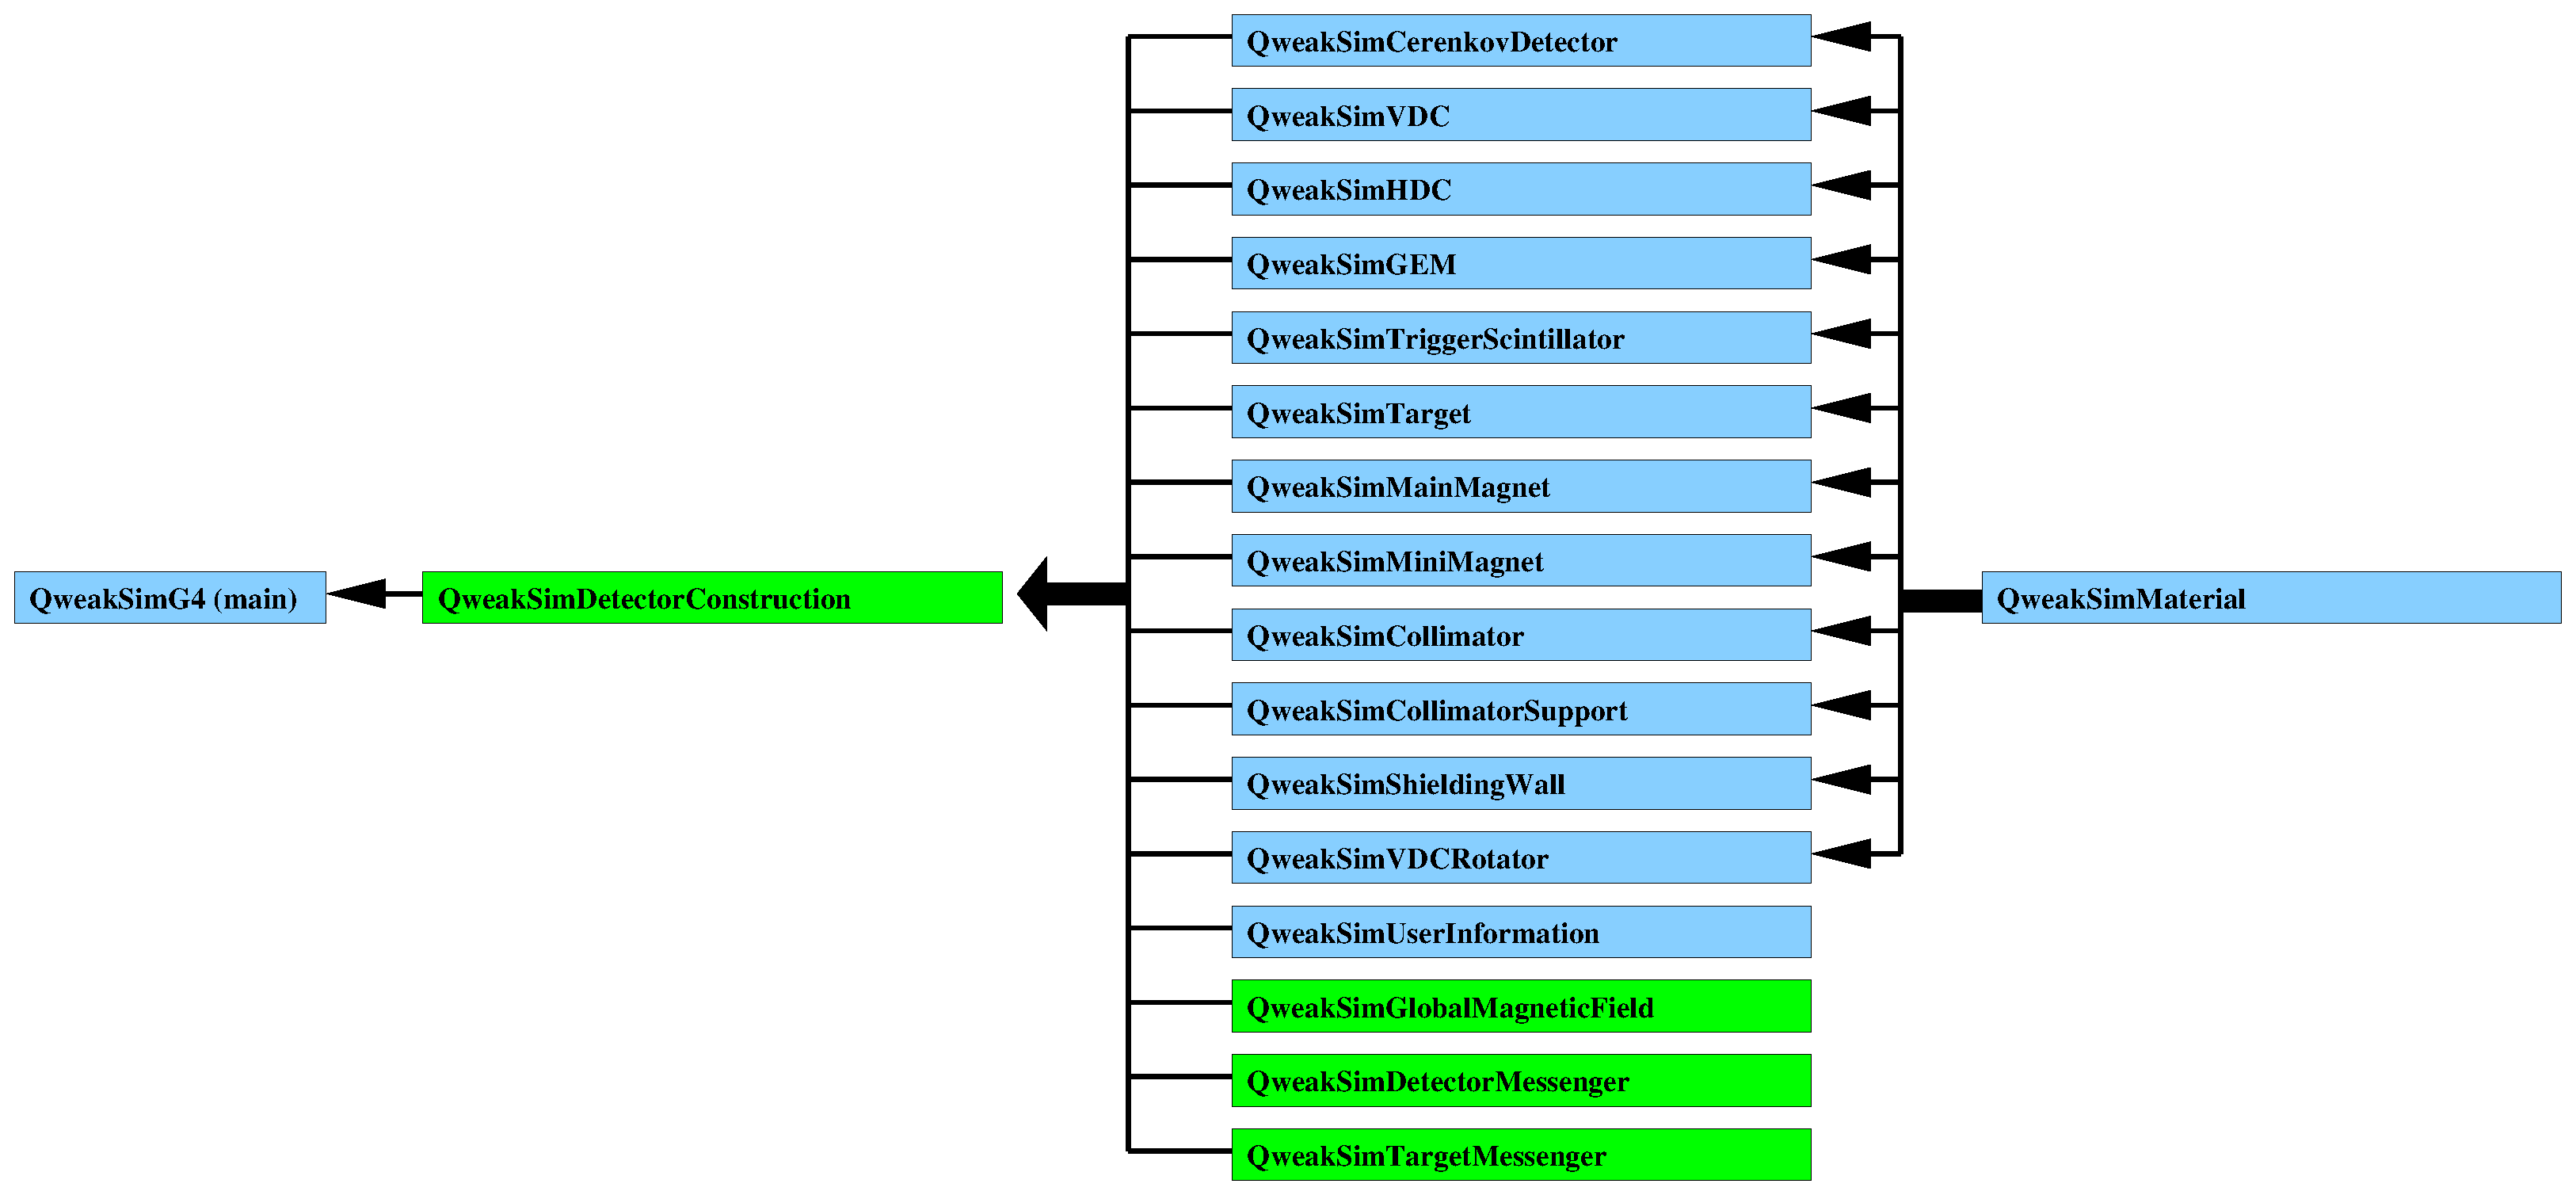
\includegraphics[scale=0.4]{./chapter1/figures/QweakSimClassTree04.eps}
  \caption{Base classes within the {\em QweakSimG4} hierarchy. The
           ``yellow'' boxes indicate classes that are turned into ROOT
           objects. They are base classes within the Qweak simulation
           framework. However, some of them are derived from the ROOT
           {\em TObject} class.  The ``blue'' boxes indicate regular
           non-ROOT (true) base classes, while the ``green'' boxes show the
           non-ROOT Qweak Simulation classes that are derived from Geant4
           classes. The latter form the main interface to the simulation
           engine, prodividing it with the geometry, the physics, tracking 
           and information about sensitive detectors as well as hit counting.}
           \label{fig:CLTR1}
\end{figure}

\clearpage

\begin{landscape}
\begin{figure}[h]
  \hspace{0cm}
  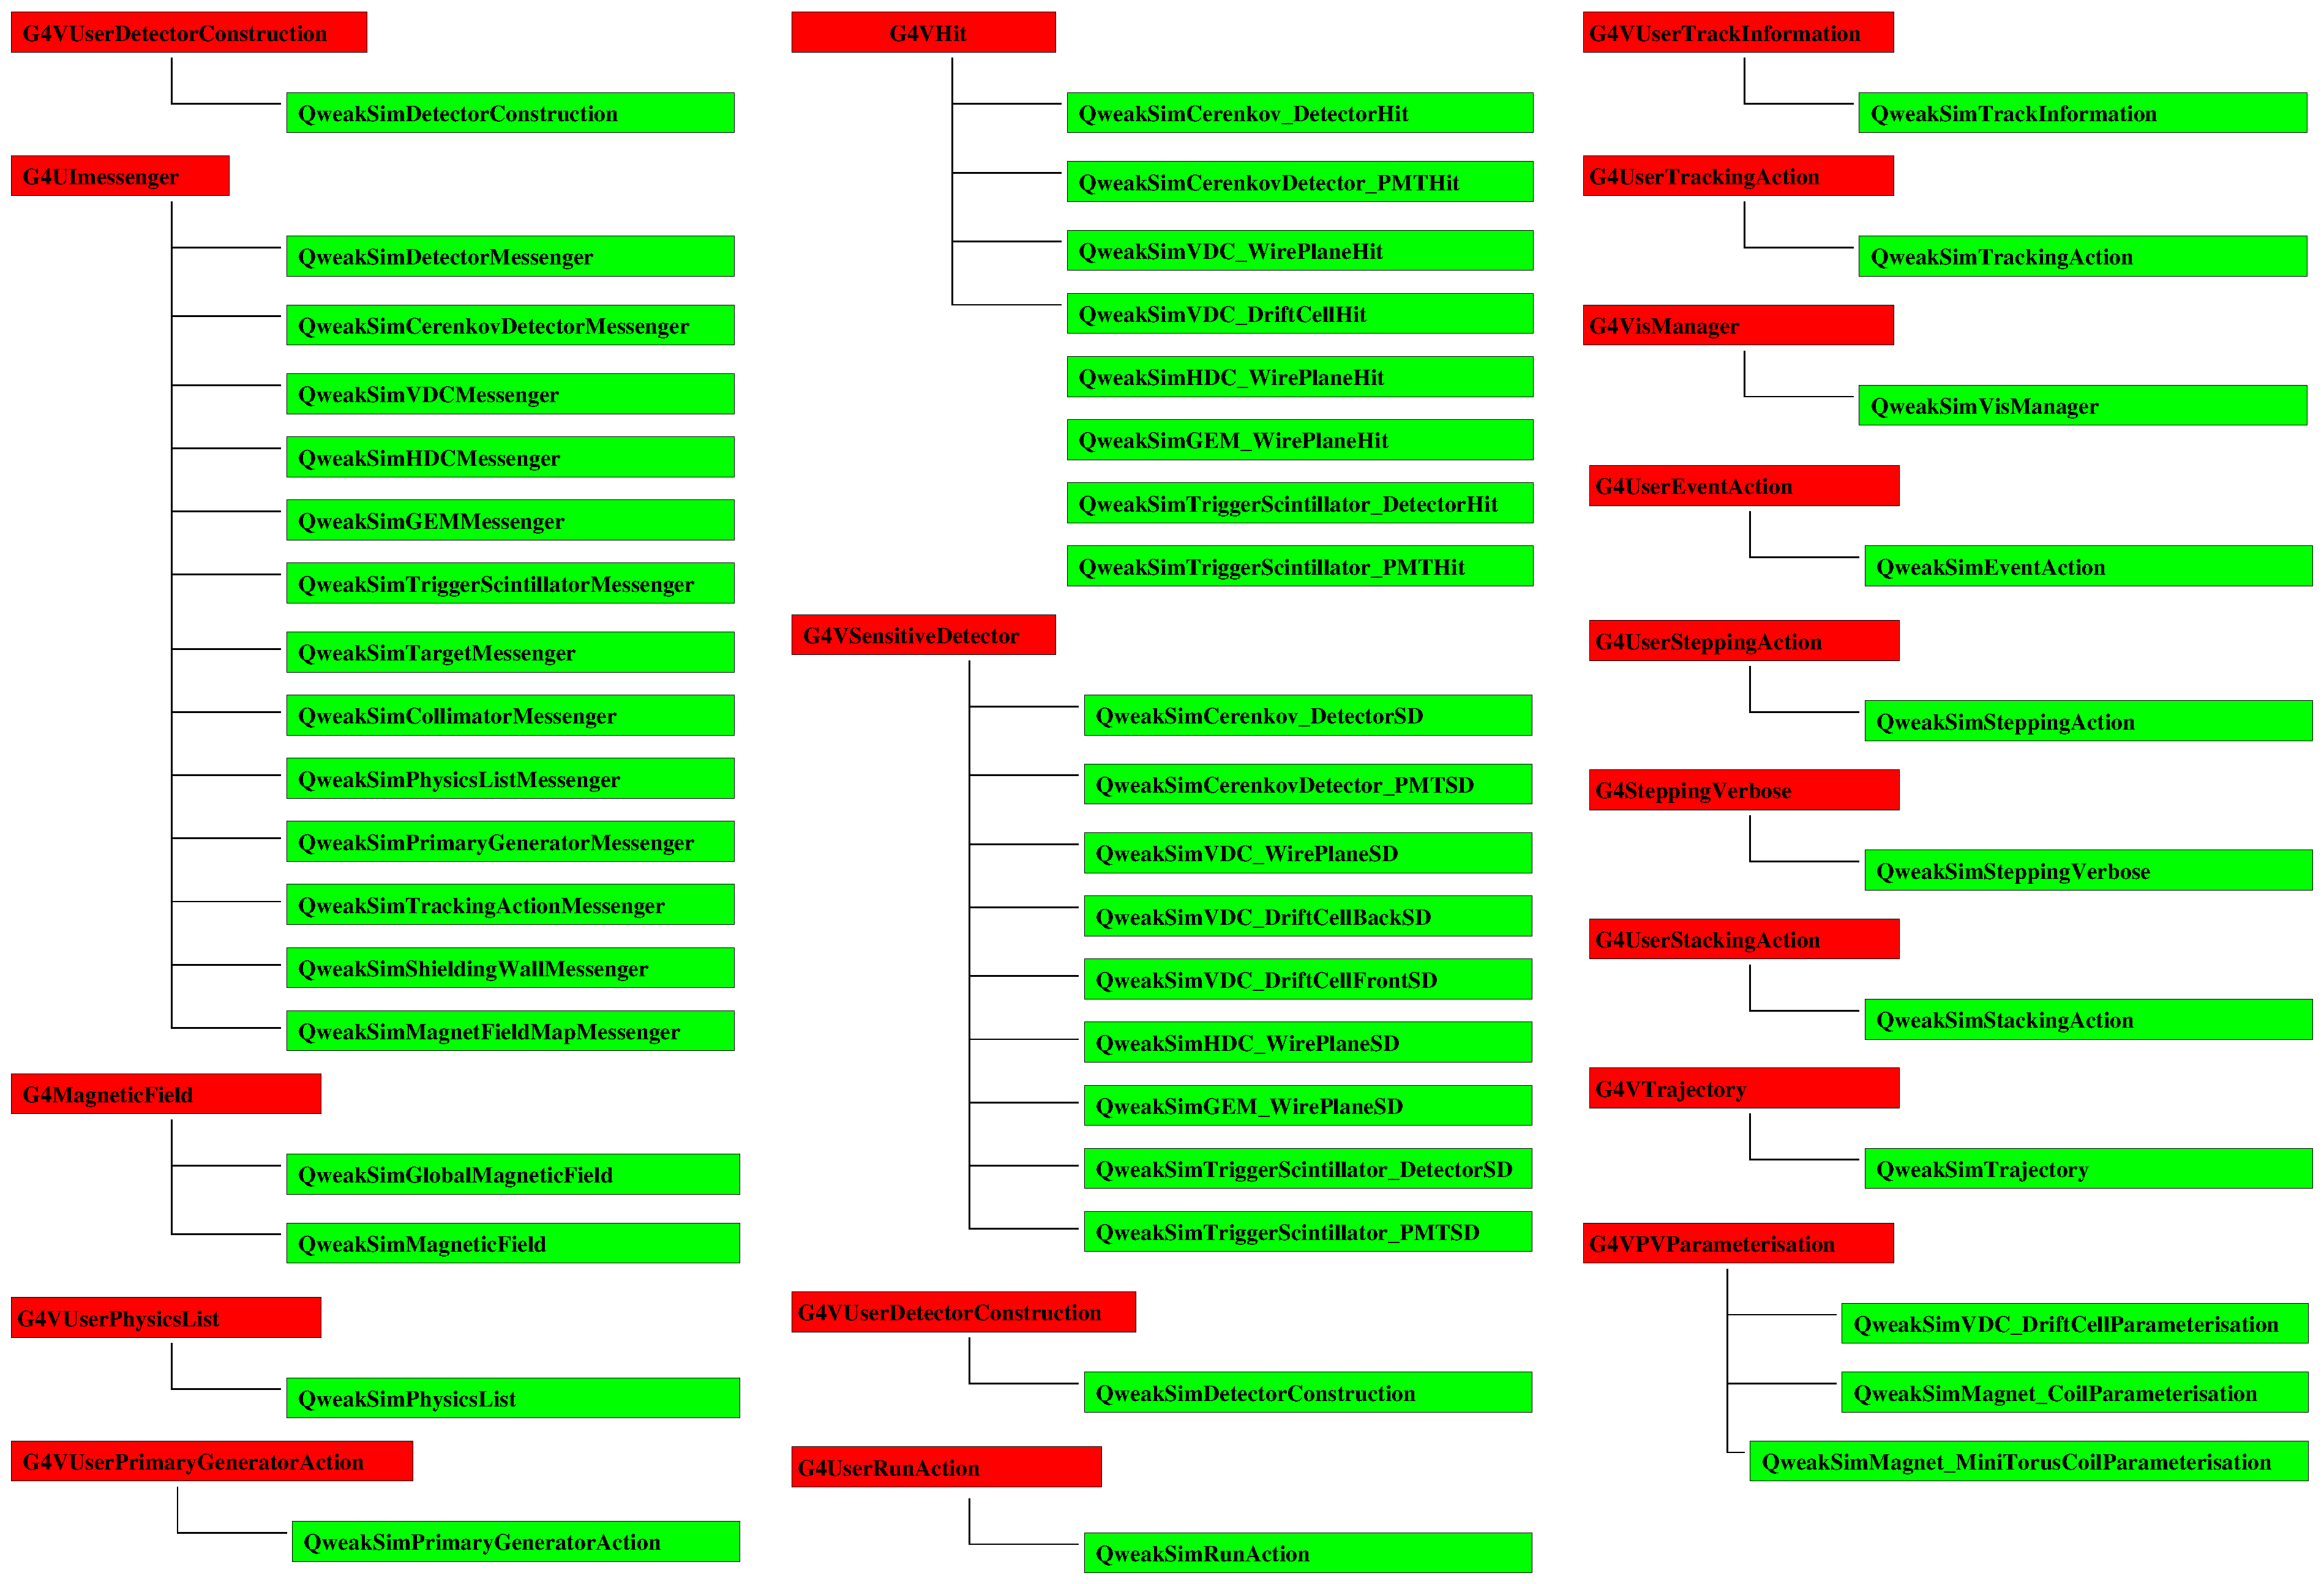
\includegraphics[scale=0.34]{./chapter1/figures/QweakSimClassTree01.eps}
%  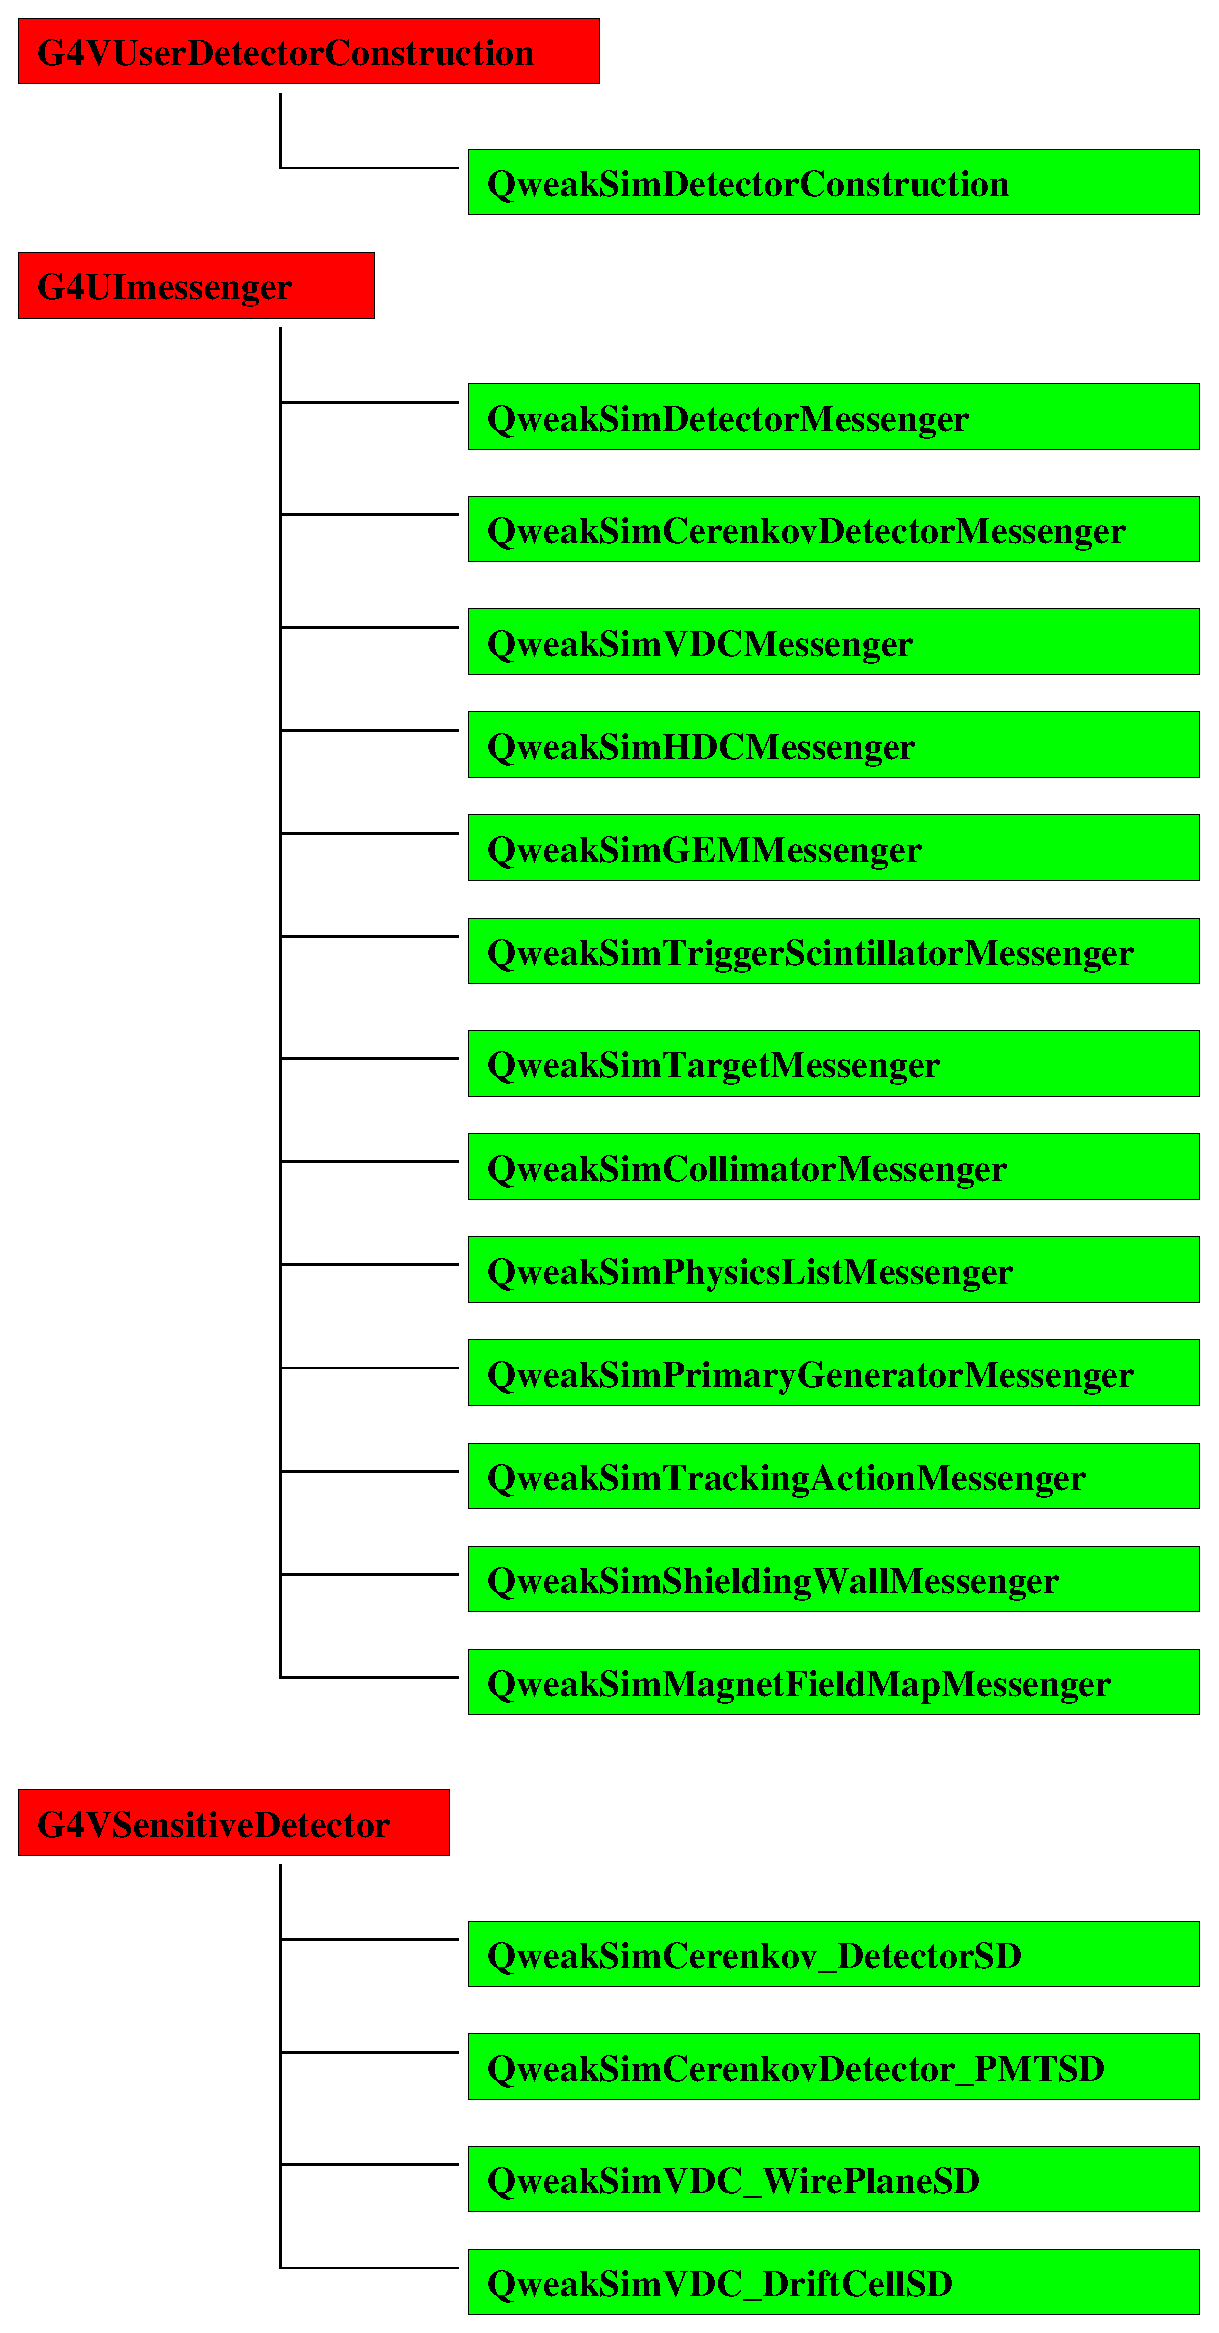
\includegraphics[scale=0.36]{./chapter1/figures/QweakSimClassTree02.eps}
%  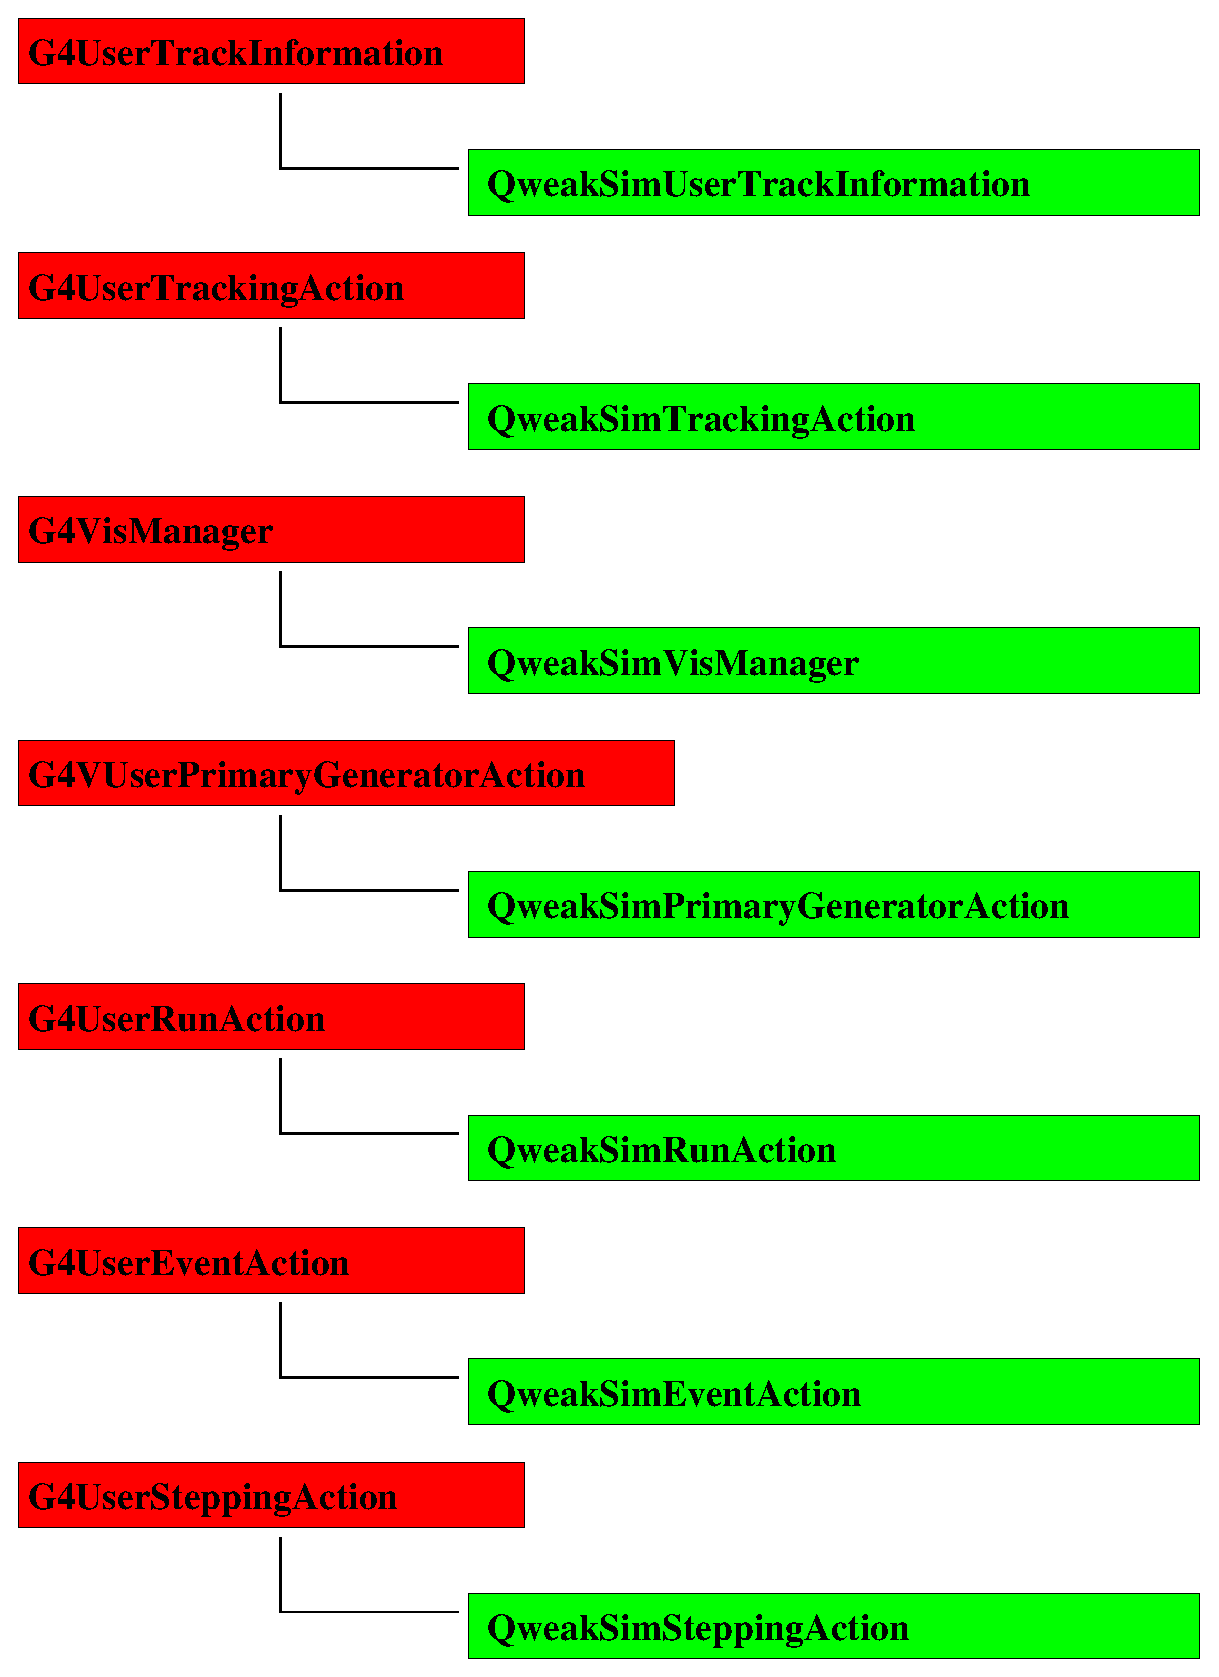
\includegraphics[scale=0.36]{./chapter1/figures/QweakSimClassTree03.eps}
  \caption{Class hierarchy within the {\em QweakSimG4} program. The ``red''
           boxes indicate GEANT4 classes.}
           \label{fig:CLTR2}
\end{figure}

\end{landscape}
\clearpage

Figure ~\ref{fig:CLDP} shows the interdependence of the classes. That
is, one ore more instances of a class object is used in some other
class.  This is different from class interdependence due to
inheritance. Each class in the library has a reasonably well defined
purpose and the class names are supposed to be indicative of this
purpose. The details for each class are described in chapter the
following chapters, including their overall purpose and an explanation
of their member functions and data members.


\section{Preliminaries: Installing Geant4 with Coin3D and ROOT} \label{CHP_I-SCN_II}

This simulation package requires a LINUX operating system (MAC should
work, Windows only via Cygwin) with the ROOT libraries and programs
installed. In addition, you need the OpenGL (or mesa) libraries and
source code (including the development libraries). Your search path
should contain the directory with the correct ROOT installation.

For example, for the {\em bash} shell you should have the following
statements in your {\em .bashrc} file:
\begin{verbatim}
export ROOTSYS=/usr/local/root
export PATH=$ROOTSYS/bin:$PATH
\end{verbatim}
You should also have defined the correct library path, as in:
\begin{verbatim}
export LD_LIBRARY_PATH=$ROOTSYS/lib:$LD_LIBRARY_PATH 
\end{verbatim}
But if ROOT is currently running on your system, these should be already
defined somwhere.

Also, the successful installation of Geant4 itself will have required
that the following switches are in your search path (this is for LINUX only),
with the directories changed accordingly:

\begin{verbatim}
######################################
#
# ROOT
#
#+

export ROOTSYS=/usr/local/root
export PATH=$ROOTSYS/bin:$PATH
export PATH=/usr/local/root/hbook:$PATH
export LD_LIBRARY_PATH=$ROOTSYS/lib:$LD_LIBRARY_PATH
export OPENGL=/usr
export MYSQL=/usr

######################################
#
# OpenInventor and Coin3D
#
#+

export COIN=/usr/local/Coin3D
export PATH=$COIN/bin:$PATH
export OIVHOME=$COIN
export SOXT=/usr/local/SoXt
export OIVFLAGS="-I$COIN/include -DINVENTOR2_1 -I$SOXT/include"
export OIVLIBS="-L$COIN/lib -lCoin -L$SOXT/lib -lSoXt"
export LD_LIBRARY_PATH=$LD_LIBRARY_PATH:$COIN/lib:$SOXT/lib
export COIN_FULL_INDIRECT_RENDERING=1


######################################
#
# GEANT4
#
#+

export G4SYSTEM="Linux-g++"
export G4INSTALL=/usr/local/geant4.8.2
export G4INCLUDE=/usr/local/geant4.8.2/include
export G4LIB=/usr/local/geant4.8.2/lib
export G4LEVELGAMMADATA=/usr/local/geant4.8.2/data/PhotonEvaporation2.0
export G4RADIOACTIVEDATA=/usr/local/geant4.8.2/data/RadiativeDecay3.1
export G4LEDATA=/usr/local/geant4.8.2/data/G4EMLOW4.2
export NeutronHPCrossSections=/usr/local/geant4.8.2/data/G4NDL3.10
export G4ELASTICDATA=/usr/local/geant4.8.2/data/G4ELASTIC1.1
export CLHEP_BASE_DIR=/usr/local
export CLHEP_INCLUDE_DIR=/usr/local/include
export CLHEP_LIB_DIR=/usr/local/lib
export CLHEP_LIB=CLHEP
export G4LISTS_BASE=$G4LIB

export G4VIS_BUILD_OIX_DRIVER=1
export G4VIS_USE_OIX=1

export G4VIS_BUILD_DAWN_DRIVER=1
export G4VIS_USE_DAWN=1

export G4VIS_BUILD_OPENGLX_DRIVER=1
export G4VIS_USE_OPENGLX=1
export OGLHOME=/usr
export OGLFLAGS="-I$OGLHOME/include/GL"
export OGLFLAGS="-I$OGLHOME/lib"
export G4VIS_BUILD_OGLIX_DRIVER=1
export G4VIS_USE_OGLIX=1
export G4UI_USE_XM=1
export G4UI_BUILD_XM_SESSION=1

export G4VIS_BUILD_VRML_DRIVER=1
export G4VIS_USE_VRML=1
export G4LIB_BUILD_SHARED=1
export G4LIB_USE_GRANULAR=1

export G4UI_USE_TCSH=1
export G4ANALYSIS_USE=1
export G4LIB_BUILD_G3TOG4=1
export G4LIB_USE_G3TOG4=1
export G4LIB_USE_ZLIB=1

export LD_LIBRARY_PATH=$CLHEP_BASE_DIR/lib:$LD_LIBRARY_PATH
export LD_LIBRARY_PATH=$G4LIB:$LD_LIBRARY_PATH
export LD_LIBRARY_PATH=$G4LIB/$G4SYSTEM:$LD_LIBRARY_PATH$
\end{verbatim}

For visualization, the installation of Coin3D is desired.
While there are other forms of visualization that can be used,
this appears to be the most versatile and is relatively easy
to use. The process to install Geant4 with Coin3D is outlined
below.

\begin{enumerate}
  \item{http://www.coin3d.org and follow the Download link of Coin3D}
  \item{Copy and unpack into some source directory, like \\
       {\em /usr/local/src/Coin3D/Coin-2.4.5} \\
       or whatever current version it is.}
  \item{Run: {\em ./configure --prefix=/usr/local/Coin3D/Coin-2.4.5} \\
        and note that the installation directory should be different
        from the source directory.}
  \item{Run: {\em make install} \\ Which compiles Coin3D and generates
        includes, binaries, and libraries in {\em /usr/local/Coin3D/Coin-2.4.5}}
  \item{Download the SoXt package from the Coin3D site.}
  \item{Copy and unpack into the source directory \\
       {\em /usr/local/src/Coin3D/SoXt-1.2.2} \\
       or whatever current version it is.}
  \item{Run: {\em ./configure --prefix=/usr/local/Coin3D/SoXt-1.2.2} \\
        and note that the installation directory should be different
        from the source directory.}
  \item{Run: {\em make install} \\ Which compiles SoXt and generates
        includes, binaries, and libraries in {\em /usr/local/Coin3D/SoXt-1.2.2}}
  \item{Update your environment (see above).}
  \item{Compile (or recompile) Geant4. \\
        Be sure that your xterm window (in which you will compile Geant4)
        knows about the updated environment settings
        (e.g. do a "source ~/.bashrc) \\ \\
	Important: Before compiling Geant4, modify the following Geant4 file: \\
        {\em G4INSTALL/config/sys/Linux-g++.gmk} \\
        remove "-pedantic" \\
	It should look now like this:
	\begin{verbatim}
	# CXXFLAGS := -W -Wall -ansi -pedantic -Wno-non-virtual-dtor-Wno-long-long
	CXXFLAGS := -W -Wall -ansi           -Wno-non-virtual-dtor-Wno-long-long
	\end{verbatim}
        }
\end{enumerate}

\section{Compiling QweakSim}

The source code is availabe as an archive (a gzipped {\em tar} file)
from the Qweak simulation logbook\footnote{{\tt
http://dilbert.physics.wm.edu/elog/Software/}} or via CVS (put info
here). Upon downloading the archive and placing it in a directory of
your choice, unload the archive by typing at the LINUX terminal
prompt:
\begin{verbatim}
tar -xvzf qweaksim.tar.gz
\end{verbatim}
This should create the directories {\em ./include}, {\em ./src}, and
{\em Documentation}. Create a directiry called {\em tmp}:
\begin{verbatim}
mkdir tmp
\end{verbatim}
Set your current working directory:
\begin{verbatim}
export G4WORKDIR=`pwd`
export G4TMP=`pwd`/tmp
\end{verbatim}
Compile the simulation:
\begin{verbatim}
make clean
make
\end{verbatim}

\section{Running the Simulation}

After the very first compilationof the simulation: make a symbolic link to the binary
\begin{verbatim}
ln -s bin/Linux-g++/QweakSimG4 QweakSimG4
\end{verbatim}
Also make symbolic links to the field maps (wherever they are located):
\begin{verbatim}
ln -s ../MagnetFieldMaps/MainMagnet_FieldMap.dat MainMagnet_FieldMap.dat
ln -s ../MagnetFieldMaps/MiniTorus_FieldMap.dat  MiniTorus_FieldMap.dat
\end{verbatim}
Also make a symbolic link to the primary event file:
\begin{verbatim}
ln -s  ../PrimaryEvents/ROOT/v5.08/ep_m84_qweak_final.root ep_elastic.root
\end{verbatim}
Finally, the simulation is started with the following commands

For visualization with new events, using Coin3D
\begin{verbatim}
   ./QweakSimG4 > mylogfile.txt                  
\end{verbatim}
    
For running with several k events without visualization
\begin{verbatim}
./QweakSimG4 myRun.mac > /dev/zero 
\end{verbatim}
     

\subsection{Using the visualization}
Executing  the command:
\begin{verbatim}
./QweakSimG4 > mylogfile.txt 
\end{verbatim}
will open a G4UIXm window for steering the simulation.

Within this window click on:
\begin{verbatim}
Vis->myVis.mac (OIX)
\end{verbatim}
This will execute the Geant4 input file {\em myVis.mac} which will
open a Coin3D window for geometry/track visualization.
The Coin3D is black/blank initially. Click in the Coin3D window on,
\begin{verbatim}
Etc->visible mother + visible daughters
\end{verbatim} 
which will then display the geometry.
 
Click 
\begin{verbatim}
  Help->Controls
\end{verbatim} 
for how to use the mouse pointer or the wheels for rotating, zooming, or moving the geometry.

Back in the G4UIXm you can change parameters of the simulation:
click on 
\begin{verbatim}
 DetectorHut->ShowTopWall
\end{verbatim} 
then click in Coin3D on 
\begin{verbatim}
Etc->visible mother + visible daughters
\end{verbatim} 
Click on 
\begin{verbatim}
TrackingAction->Track primaries only
\end{verbatim} 
this will track/transport only the primary electrons, as defined by
the event generator (root-file). By default, secondaries are produced 
but not tracked.
 
After you have selected your options, click finally on 
\begin{verbatim}
  Run->beamOn X
\end{verbatim} 
to start the simulation. 

If, in Coin3D, the screen gets erased, again select 
\begin{verbatim}
  Etc->visible mother + visible daughters
\end{verbatim} 
for displaying geometry and tracks.  In addition you might erase
tracks and/or geometry in Coin3D using 
\begin{verbatim}
  Etc->Erase event
\end{verbatim} 
or
\begin{verbatim}
Etc->Erase detector 
\end{verbatim}

Beware that selecting more than 100 tracks will significantly slow
down the visualization, depending on the speed of your machine.
